\section{eo\-Es\-Chrom\-Init$<$ EOT $>$ Class Template Reference}
\label{classeo_es_chrom_init}\index{eoEsChromInit@{eoEsChromInit}}
Random Es-chromosome initializer (therefore derived from {\bf eo\-Init}{\rm (p.\,\pageref{classeo_init})}).  


{\tt \#include $<$eo\-Es\-Chrom\-Init.h$>$}

Inheritance diagram for eo\-Es\-Chrom\-Init$<$ EOT $>$::\begin{figure}[H]
\begin{center}
\leavevmode
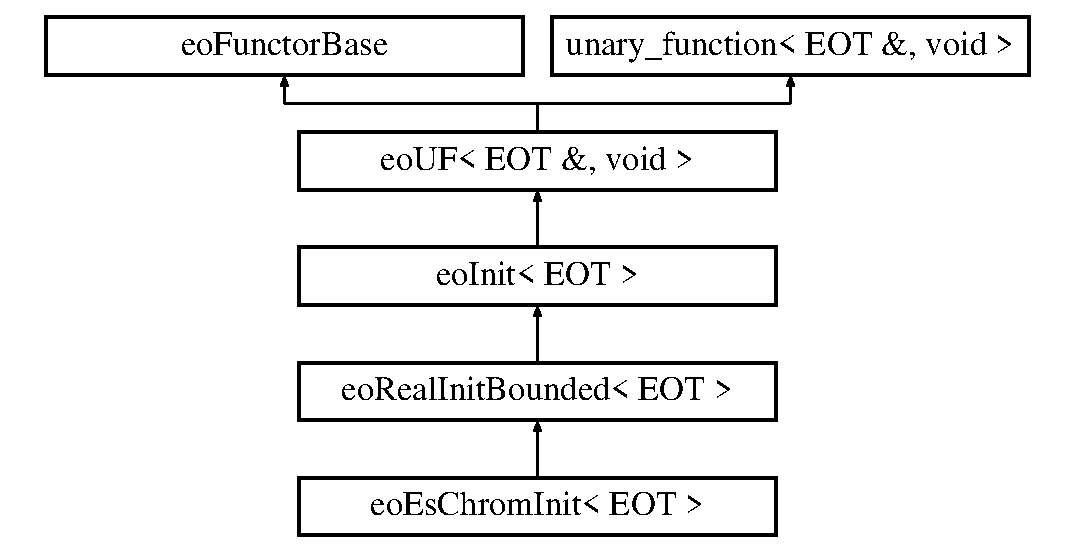
\includegraphics[height=5cm]{classeo_es_chrom_init}
\end{center}
\end{figure}
\subsection*{Public Types}
\begin{CompactItemize}
\item 
typedef EOT::Fitness {\bf Fit\-T}\label{classeo_es_chrom_init_w0}

\end{CompactItemize}
\subsection*{Public Member Functions}
\begin{CompactItemize}
\item 
{\bf eo\-Es\-Chrom\-Init} ({\bf eo\-Real\-Vector\-Bounds} \&\_\-bounds, double \_\-sigma=0.3, bool \_\-to\_\-scale=false)
\begin{CompactList}\small\item\em Constructor. \item\end{CompactList}\item 
{\bf eo\-Es\-Chrom\-Init} ({\bf eo\-Real\-Vector\-Bounds} \&\_\-bounds, std::vector$<$ double $>$ \_\-vec\-Sigma)
\begin{CompactList}\small\item\em Constructor. \item\end{CompactList}\item 
void {\bf operator()} ({\bf EOT} \&\_\-eo)\label{classeo_es_chrom_init_a2}

\begin{CompactList}\small\item\em simply passes the argument to the uniform method of the bounds \item\end{CompactList}\end{CompactItemize}
\subsection*{Private Member Functions}
\begin{CompactItemize}
\item 
void {\bf create\_\-self\_\-adapt} ({\bf eo\-Real}$<$ Fit\-T $>$ \&)
\begin{CompactList}\small\item\em Create intializer. \item\end{CompactList}\item 
void {\bf create\_\-self\_\-adapt} ({\bf eo\-Es\-Simple}$<$ Fit\-T $>$ \&result)
\begin{CompactList}\small\item\em Create intializer. \item\end{CompactList}\item 
void {\bf create\_\-self\_\-adapt} ({\bf eo\-Es\-Stdev}$<$ Fit\-T $>$ \&result)
\begin{CompactList}\small\item\em Create intializer. \item\end{CompactList}\item 
void {\bf create\_\-self\_\-adapt} ({\bf eo\-Es\-Full}$<$ Fit\-T $>$ \&result)
\begin{CompactList}\small\item\em Create intializer. \item\end{CompactList}\end{CompactItemize}
\subsection*{Private Attributes}
\begin{CompactItemize}
\item 
double {\bf unique\-Sigma}\label{classeo_es_chrom_init_r0}

\begin{CompactList}\small\item\em Initial value in case of a unique sigma. \item\end{CompactList}\item 
std::vector$<$ double $>$ {\bf vec\-Sigma}\label{classeo_es_chrom_init_r1}

\begin{CompactList}\small\item\em Initial values in case of a vector of sigmas. \item\end{CompactList}\end{CompactItemize}


\subsection{Detailed Description}
\subsubsection*{template$<$class EOT$>$ class eo\-Es\-Chrom\-Init$<$ EOT $>$}

Random Es-chromosome initializer (therefore derived from {\bf eo\-Init}{\rm (p.\,\pageref{classeo_init})}). 

This class can initialize four types of real-valued genotypes thanks to tempate specialization of private method create:

\begin{itemize}
\item {\bf eo\-Real}{\rm (p.\,\pageref{classeo_real})} just an eo\-Vector$<$double$>$\item {\bf eo\-Es\-Simple}{\rm (p.\,\pageref{classeo_es_simple})} + one self-adapting single sigma for all variables\item {\bf eo\-Es\-Stdev}{\rm (p.\,\pageref{classeo_es_stdev})} a whole std::vector of self-adapting sigmas\item {\bf eo\-Es\-Full}{\rm (p.\,\pageref{classeo_es_full})} a full self-adapting correlation matrix\end{itemize}


\begin{Desc}
\item[See also:]{\bf eo\-Real}{\rm (p.\,\pageref{classeo_real})} {\bf eo\-Es\-Simple}{\rm (p.\,\pageref{classeo_es_simple})} {\bf eo\-Es\-Stdev}{\rm (p.\,\pageref{classeo_es_stdev})} {\bf eo\-Es\-Full}{\rm (p.\,\pageref{classeo_es_full})} {\bf eo\-Init}{\rm (p.\,\pageref{classeo_init})} \end{Desc}




Definition at line 55 of file eo\-Es\-Chrom\-Init.h.

\subsection{Constructor \& Destructor Documentation}
\index{eoEsChromInit@{eo\-Es\-Chrom\-Init}!eoEsChromInit@{eoEsChromInit}}
\index{eoEsChromInit@{eoEsChromInit}!eoEsChromInit@{eo\-Es\-Chrom\-Init}}
\subsubsection{\setlength{\rightskip}{0pt plus 5cm}template$<$class EOT$>$ {\bf eo\-Es\-Chrom\-Init}$<$ {\bf EOT} $>$::{\bf eo\-Es\-Chrom\-Init} ({\bf eo\-Real\-Vector\-Bounds} \& {\em \_\-bounds}, double {\em \_\-sigma} = {\tt 0.3}, bool {\em \_\-to\_\-scale} = {\tt false})\hspace{0.3cm}{\tt  [inline]}}\label{classeo_es_chrom_init_a0}


Constructor. 

\begin{Desc}
\item[Parameters:]
\begin{description}
\item[{\em \_\-bounds}]bounds for uniform initialization \item[{\em \_\-sigma}]initial value for the stddev \item[{\em \_\-to\_\-scale}]wether sigma should be multiplied by the range of each variable added December 2004 - MS (together with the whole comment :-) \end{description}
\end{Desc}


Definition at line 71 of file eo\-Es\-Chrom\-Init.h.

References eo\-Real\-Base\-Vector\-Bounds::range(), eo\-Real\-Init\-Bounded$<$ EOT $>$::the\-Bounds(), eo\-Es\-Chrom\-Init$<$ EOT $>$::unique\-Sigma, and eo\-Es\-Chrom\-Init$<$ EOT $>$::vec\-Sigma.\index{eoEsChromInit@{eo\-Es\-Chrom\-Init}!eoEsChromInit@{eoEsChromInit}}
\index{eoEsChromInit@{eoEsChromInit}!eoEsChromInit@{eo\-Es\-Chrom\-Init}}
\subsubsection{\setlength{\rightskip}{0pt plus 5cm}template$<$class EOT$>$ {\bf eo\-Es\-Chrom\-Init}$<$ {\bf EOT} $>$::{\bf eo\-Es\-Chrom\-Init} ({\bf eo\-Real\-Vector\-Bounds} \& {\em \_\-bounds}, std::vector$<$ double $>$ {\em \_\-vec\-Sigma})\hspace{0.3cm}{\tt  [inline]}}\label{classeo_es_chrom_init_a1}


Constructor. 

This is an overloaded member function, provided for convenience. It differs from the above function only in what argument(s) it accepts.

Specify individual initial sigmas for each variable.

\begin{Desc}
\item[Parameters:]
\begin{description}
\item[{\em \_\-bounds}]bounds for uniform initialization \item[{\em \_\-sigma}]initial value for the stddev \end{description}
\end{Desc}


Definition at line 109 of file eo\-Es\-Chrom\-Init.h.

References eo\-Es\-Chrom\-Init$<$ EOT $>$::unique\-Sigma, and eo\-Es\-Chrom\-Init$<$ EOT $>$::vec\-Sigma.

\subsection{Member Function Documentation}
\index{eoEsChromInit@{eo\-Es\-Chrom\-Init}!create_self_adapt@{create\_\-self\_\-adapt}}
\index{create_self_adapt@{create\_\-self\_\-adapt}!eoEsChromInit@{eo\-Es\-Chrom\-Init}}
\subsubsection{\setlength{\rightskip}{0pt plus 5cm}template$<$class EOT$>$ void {\bf eo\-Es\-Chrom\-Init}$<$ {\bf EOT} $>$::create\_\-self\_\-adapt ({\bf eo\-Real}$<$ Fit\-T $>$ \&)\hspace{0.3cm}{\tt  [inline, private]}}\label{classeo_es_chrom_init_d0}


Create intializer. 

No adaptive mutation at all 

Definition at line 128 of file eo\-Es\-Chrom\-Init.h.

Referenced by eo\-Es\-Chrom\-Init$<$ EOT $>$::operator()().\index{eoEsChromInit@{eo\-Es\-Chrom\-Init}!create_self_adapt@{create\_\-self\_\-adapt}}
\index{create_self_adapt@{create\_\-self\_\-adapt}!eoEsChromInit@{eo\-Es\-Chrom\-Init}}
\subsubsection{\setlength{\rightskip}{0pt plus 5cm}template$<$class EOT$>$ void {\bf eo\-Es\-Chrom\-Init}$<$ {\bf EOT} $>$::create\_\-self\_\-adapt ({\bf eo\-Es\-Simple}$<$ Fit\-T $>$ \& {\em result})\hspace{0.3cm}{\tt  [inline, private]}}\label{classeo_es_chrom_init_d1}


Create intializer. 

This is an overloaded member function, provided for convenience. It differs from the above function only in what argument(s) it accepts.

Adaptive mutation through a unique sigma 

Definition at line 139 of file eo\-Es\-Chrom\-Init.h.

References eo\-Es\-Simple$<$ Fit $>$::stdev.\index{eoEsChromInit@{eo\-Es\-Chrom\-Init}!create_self_adapt@{create\_\-self\_\-adapt}}
\index{create_self_adapt@{create\_\-self\_\-adapt}!eoEsChromInit@{eo\-Es\-Chrom\-Init}}
\subsubsection{\setlength{\rightskip}{0pt plus 5cm}template$<$class EOT$>$ void {\bf eo\-Es\-Chrom\-Init}$<$ {\bf EOT} $>$::create\_\-self\_\-adapt ({\bf eo\-Es\-Stdev}$<$ Fit\-T $>$ \& {\em result})\hspace{0.3cm}{\tt  [inline, private]}}\label{classeo_es_chrom_init_d2}


Create intializer. 

This is an overloaded member function, provided for convenience. It differs from the above function only in what argument(s) it accepts.

Adaptive mutation through a std::vector of sigmas

\begin{Desc}
\item[{\bf Todo}]Should we scale sigmas to the corresponding object variable range? \end{Desc}


Definition at line 155 of file eo\-Es\-Chrom\-Init.h.

References eo\-Es\-Stdev$<$ Fit $>$::stdevs.\index{eoEsChromInit@{eo\-Es\-Chrom\-Init}!create_self_adapt@{create\_\-self\_\-adapt}}
\index{create_self_adapt@{create\_\-self\_\-adapt}!eoEsChromInit@{eo\-Es\-Chrom\-Init}}
\subsubsection{\setlength{\rightskip}{0pt plus 5cm}template$<$class EOT$>$ void {\bf eo\-Es\-Chrom\-Init}$<$ {\bf EOT} $>$::create\_\-self\_\-adapt ({\bf eo\-Es\-Full}$<$ Fit\-T $>$ \& {\em result})\hspace{0.3cm}{\tt  [inline, private]}}\label{classeo_es_chrom_init_d3}


Create intializer. 

This is an overloaded member function, provided for convenience. It differs from the above function only in what argument(s) it accepts.

Adaptive mutation through a whole correlation matrix 

Definition at line 169 of file eo\-Es\-Chrom\-Init.h.

References eo\-Es\-Full$<$ Fit $>$::correlations, eo\-Es\-Full$<$ Fit $>$::stdevs, and eo\-Rng::uniform().

The documentation for this class was generated from the following file:\begin{CompactItemize}
\item 
eo\-Es\-Chrom\-Init.h\end{CompactItemize}
